It is not surprising that weather conditions directly impact the wind power generation. The typical input parameters for wind power prediction are wind speed, temperature, pressure and humidity \cite{WindPowerGenerationUsingANN} with the most influential factor being wind speed because it is directly converted to power in the wind turbine. The following subsection will describe the collection of this data and how it is used in the modelled 

\subsection{Input Data}
The collected data for wind power prediction is described above. This subsection will go into further detail with these parameters and show their relationship with wind production.

The relationship between hourly wind speed at Aarhus Lufthavn and hourly wind power production of DK1 is seen in figure~\ref{fig:windVsProd}. The relationship is as expected even though only one weather station is used --- the relatively small size and climate of Denmark leads to uniform weather conditions across the country SHOW IT IN PLOT!.

Even though weather data from only one station is used the relationship is as expected due to the small size Denmark. The relationship is even more clear when an average of more than one station is used DO SOMETHING.  

\begin{figure}[h!]
\centering
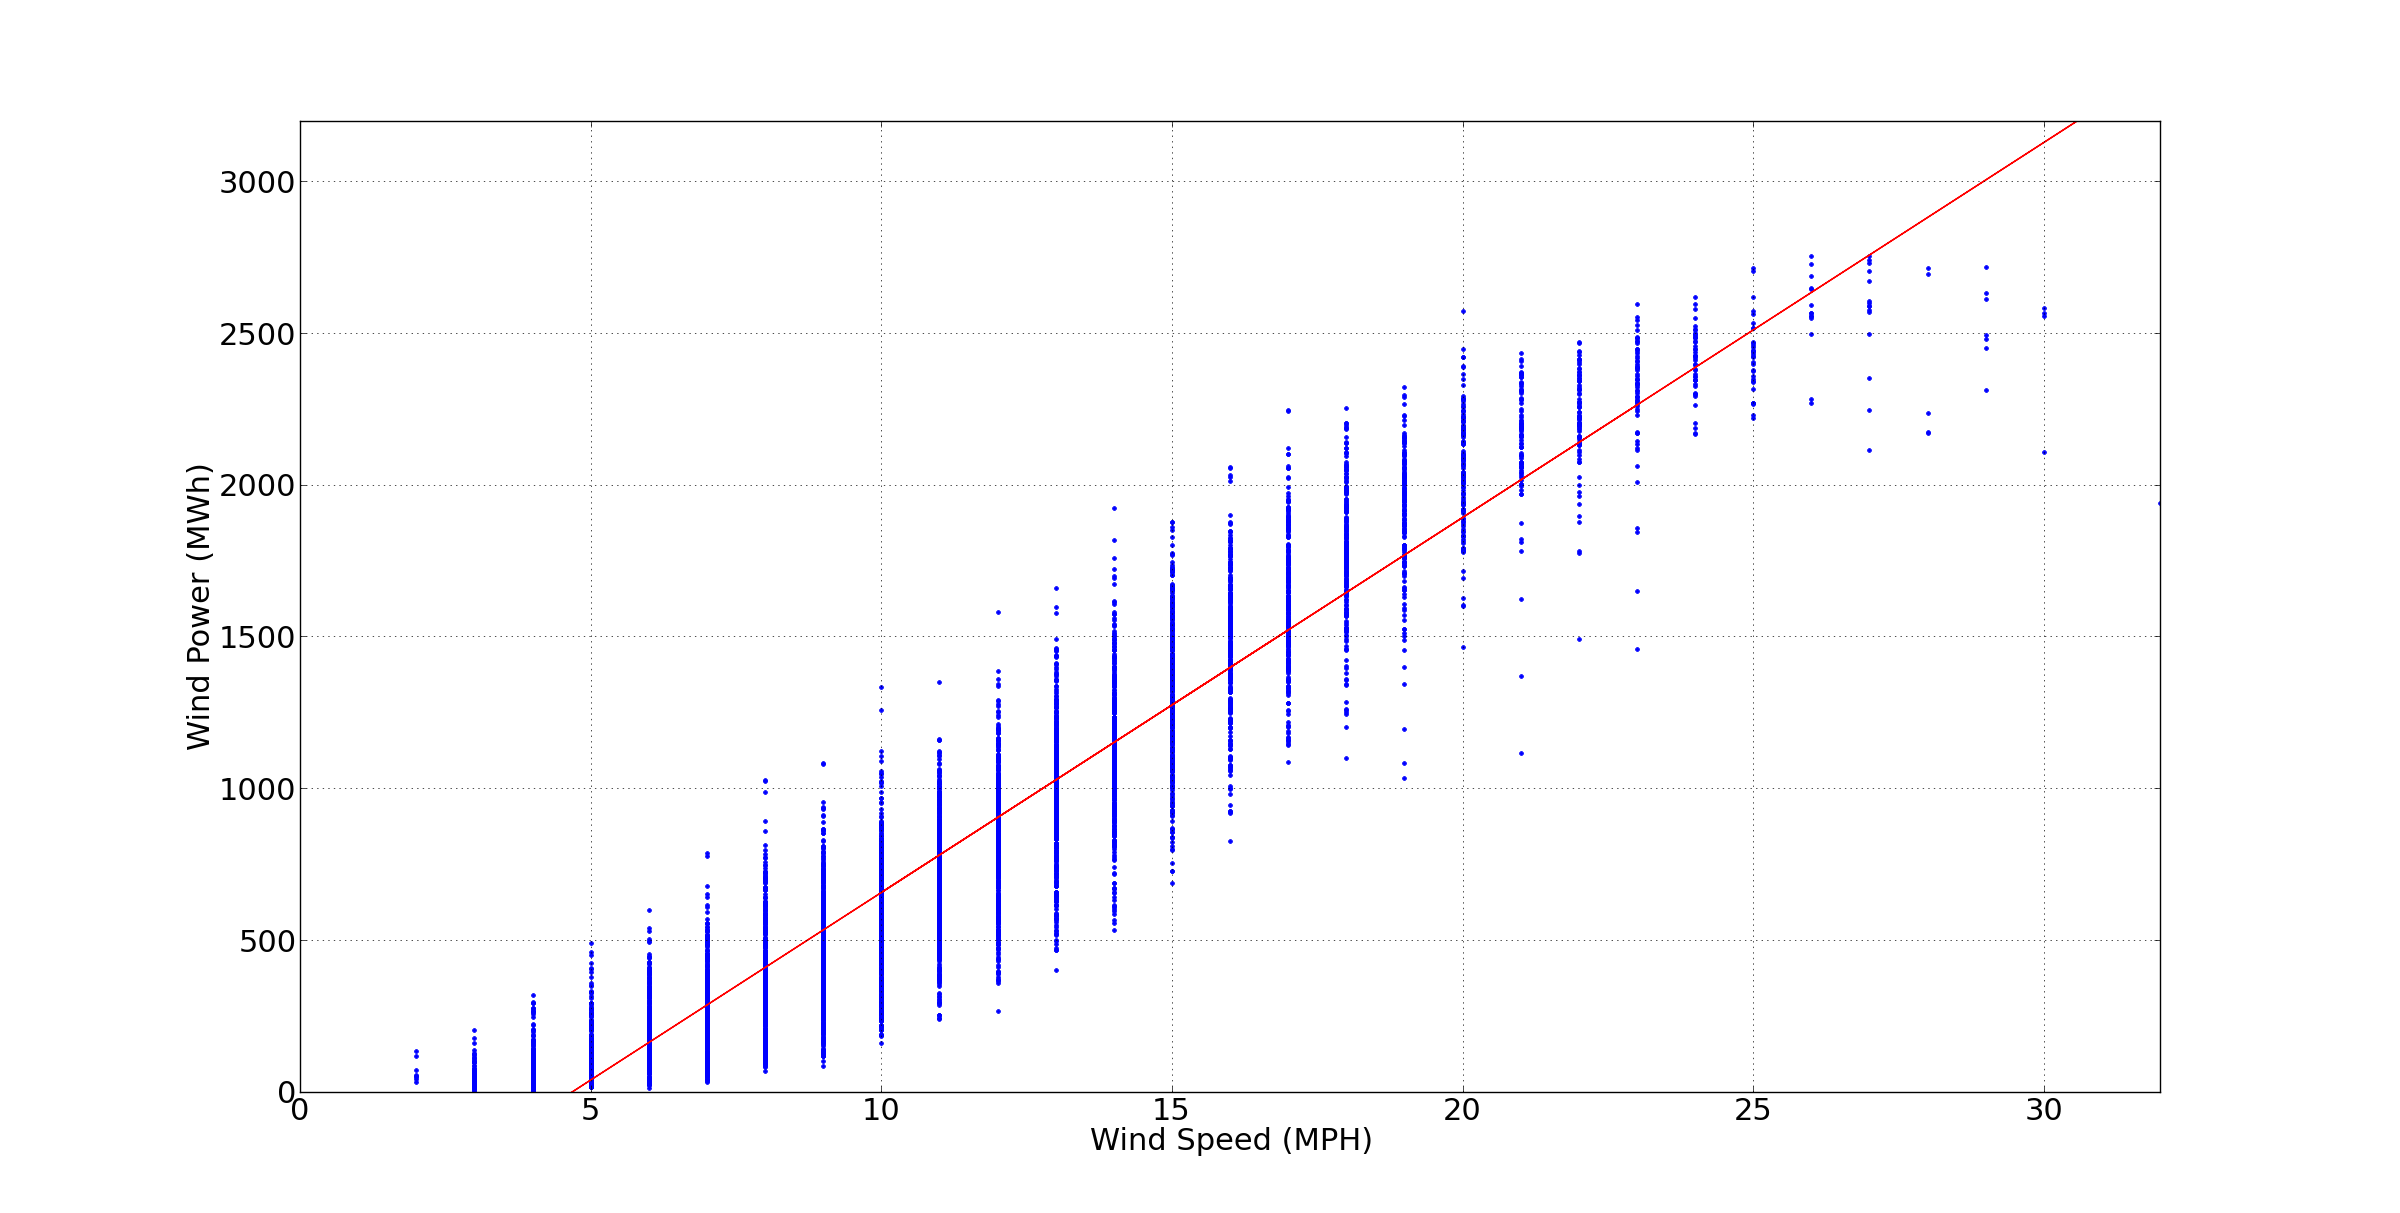
\includegraphics[width=0.99\linewidth,natwidth=898,natheight=587]{billeder/WindSpeedVsProduction.png}
\caption{Wind speed vs Wind Production}
\label{fig:windVsProd}
\end{figure}

\subsection{Modelling Artificial Neural Network}
The ANN will be trained with input the hourly parameters of wind speed, temperature, pressure and humidity and then compared to the actual production of that hour.

Black art --- experimenting with hidden layers, momentum and learning rate. 